\chapter{QoS Tools}
\section{Why QoS tools?}
In the last chapter we revised different applications with heterogeneous QoS requirements.
If all these applications coexist in the same network, it is necessary to make sure that they all see their requirements fulfilled.

One possible alternative is bandwidth overprovisioning.
If there is more than enough bandwidth, the queues are always empty and the packets suffer minimum delay and packet loss.

One of the problems of overprovisioning is that sometimes bandwidth can be very expensive.
One of the challenges of the newtwork engineers is to satisfy the QoS requirements at a reasonable cost.

Another problem of overprovisioning is the elastic demand.
Imagine that you overprovision a network to make sure that the queues are empty and the VoIP packets suffer no queueing delays.
Some users will notice that the network is blazing fast.
``Hey, I can download a HD movie in no time, I will download many of them so I can choose which one I want to watch.''
It is normal that users respond to bandwidth availability by consuming extra bandwidth.

Finally, and very similar to the previous case, there are network security threats such as worms that will consume as much bandwidth as it is available.
Sometimes a defective or misconfigured device will also consume as much bandwidth as it is available.

For all these reasons, overprovisioning cannot be the answer to everything.
An alternative to overprovisioning is to use QoS tools to manage the available bandwidth in such a way the different QoS requirements can be met by prioritizing one traffic over the others and shaping the traffic flows.

Using the road analogy, if we have an ambulances with strict delay constraints, we can make the roads wider or use prioritization and other road traffic flow management (such as traffic lamps and reversible lanes).

A QoS solution classifies the traffic into different classes accordingly to SLA requirements and treats each of these classes differently across the network.
Each of these classes is a ``class of service'' (CoS).

\section{QoS at different layers}
Our interest is on the provision of end-to-end QoS.
The layer that provides end-to-end (internetworking) connectivity is the layer 3.
In the TCP/IP stack, this is the IP layer.

Nevertheless, it is also worthy to know that Ethernet, WiFi (IEEE 802.11) and MPLS also include support for QoS.
Ethernet packets include three bits in the header (Priority Code Point, PCP) to specify the class of service.
MPLS tags also have three bits to indicate the priority. 
They are called EXP bits because they were in principle reserved for experimental use.

The case of WiFi is special because it is a shared medium, in which the different nodes contend to access the channel.
There is also support for QoS in the sense that it is possible for stations with priority packets to contend more aggressively.

IP packets have a byte for QoS.
Six of the bits are there to indicate the class of service, which is called ``differentiated services code point''.
The other two bits are for ``explicit congestion notification'' (ECN).

\section{IP flow, IP class}

IP packets can be grouped in flows.
As an example when you are browsing a webpage and send multiple HTTP request packets, all those packets belong to the same flow.
The headers of the packets of the same flow have three fields in common:

\begin{itemize}
\item The layer four protocol (either TCP or UDP)
\item The source and destination IP address
\item The source and destination port.
\end{itemize}

It is important that all the packets of a flow follow the same path and are stored in the same queues, to prevent packet re-ordering.

The number of IP flows traversing a network is humongous and therefore it is not possible to apply QoS on a per-flow basis.
The alternative is to group several flows with similar QoS requirements on the same ``Class of Service''.

As an example, all web traffic flows could be mapped to the same CoS.
Also flows from other application with similar requirements (IRC, email) could be included in the same CoS.

The millions of flows traversing a router are assigned to reasonable number of traffic classes, such as four or eight.
Then, the router treats each of these classes differently in what is known as the per-hop-behaviour PHB.

Having a reduced number of classes makes the implementation and configuration of router much more easier.
It makes it even possible to use automatic tools to configure and re-configure the routers of a network.

\section{QoS tools inside a router}

To achieve QoS end-to-end, it is necessary to provide QoS in all of the intermediate hops.
As an example, if we want to provide end-to-end bounded delay, it is required to provide  bounded delay in every single hop.

To offer QoS for a traffic class, we need to define the behaviour of the routers the networks for that class of traffic.
This is known as the per-hop-behaviour (PHB).

To implement this PHB, we will use a selection of QoS tools in each router.
Normally we will need more than one tool to achieve the goal.
Some of the tools that we will cover in the course are classifiers, meters, shapers, policers, queues and markers.

For each interface of the router, and for each direction, a chain of QoS tools is used.
An example is given in Fig. \ref{fig:qos-chain} which shows a QoS tools chain for the inbound and outbound interface of a router.

\begin{figure}[h]
\centering
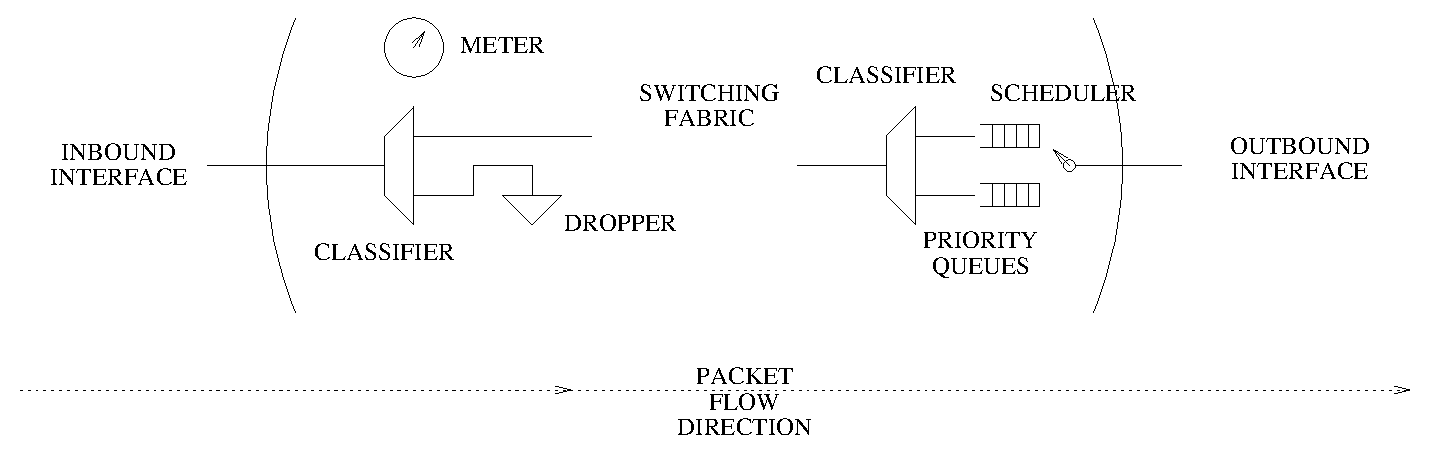
\includegraphics[width=\linewidth]{figures/qos_chain.eps}
\caption{QoS tools chain of the inbound and outbound interface of a router.}
\label{fig:qos-chain}
\end{figure}

